\documentclass[a4paper,oneside]{Tptesi2}

\usepackage[italian]{babel}
\usepackage{listings}
\usepackage{amsmath,amssymb}
\usepackage{verbatim}
\usepackage{indentfirst}
\usepackage[utf8]{inputenc}
\usepackage{subfigure}
\usepackage{algorithmic}
\usepackage{framed}
\usepackage{rotating}
\usepackage{cite}

% Packages -----------------------------------------------------------------------
%\usepackage{amsthm}
%\usepackage{amsmath}          % Non necessario se usi TPTESI2 perche' gia` incluso
%\usepackage[dvips]{graphicx}  % Non necessario se usi TPTESI2 perche' gia` incluso
%\usepackage{url} %non usare se si usa hyperref


\newcommand{\mr}{\emph{motore di ricerca}}
\newcommand{\Mr}{\emph{Motore di ricerca}}
\newcommand{\ws}{Web~service }


% Use a small font for the verbatim environment
\makeatletter  % makes '@' an ordinary character
\renewcommand{\verbatim@font}{%
  \ttfamily\footnotesize\catcode`\<=\active\catcode`\>=\active%
}
\makeatother   % makes '@' a special symbol again
%
% Simboli Matematici -------------------------------------------------------------
%\newcommand{\h}{\mathcal{H}_\infty} % scorciatoia per sequenza usata spesso
% Definizioni & Teoremi ----------------------------------------------------------
\newtheorem{teorema}{Teorema}[chapter]
\newtheorem{corollario}[teorema]{Corollario}
\newtheorem{lemma}[teorema]{Lemma}
%\theoremstyle{definition}
\newtheorem{definizione}{Definizione}[chapter]
\newtheorem{proposizione}[definizione]{Proposizione}
% Formattazione Figure -----------------------------------------------------------
\setcounter{topnumber}{3}
\setcounter{totalnumber}{3}
\def\topfraction{1}
\def\textfraction{0}
% Fuzz ---------------------------------------------------------------------------
%\hfuzz10cm %Non scassare linee che escono dal bordo
% Frontespizio -------------------------------------------------------------------
       \title{insert title\ldots}
       \author{insert candidate\ldots}
       \titolocorso{Ingegneria Informatica}
       \chair{Prof. ... \\ }
       \numberofmembers{1} %numero dei relatori
       \degreeyear{insert degree year\ldots}
       \numerocorrelatori{2} %numero dei correlatori
       \correlatori{insert correlators\ldots} % i correlatori separati da \\

%
% ---- Inclusioni (vedi piu` sotto per il comando "include" --------------
%\includeonly {introduzione,chapter1, chapter2}
%\includeonly {chapter1, chapter2, chapter3, chapter4, chapter5, chapter6}
%\includeonly{chapter6}
%
\hypersetup{%
%  pdfpagemode=FullScreen,%
  plainpages=false,%
  breaklinks,%
  pdftitle={},%
  pdfauthor={},%
  pdfsubject={},%
  pdfkeywords={},%
  colorlinks=false}

\begin{document}

\frontmatter

%\hyphenation{}
%
\pagestyle{headings} % rende attive le impostazioni sulla testata!
%
\maketitle % crea il frontespizio (ricordati di copiare "stemma.eps" nella tua directory)
%
%
%\pagenumbering{roman}
\tableofcontents % inserisce indice generale
\cleardoublepage
%\addcontentsline{toc}{chapter}{Elenco delle figure}
%\listoffigures   % inserisce indice figure
%\addcontentsline{toc}{chapter}{Elenco delle tabelle}
%\listoftables    % inserisce indice tabelle
%\addcontentsline{toc}{chapter}{Elenco degli algoritmi}
%\listofalgorithms
%
%--------------- Inizio del testo vero e proprio
%

%\cleardoublepage
%\pagenumbering{arabic}
%\input{files/ringraziamenti}
\frontmatter
\chapter{Introduzione}\label{ch:introduzione}
GUARDARE L'ABSTARCT DEL PAPER FORNITO DAL PROFESSORE 
\ldots
\cite{gruntzig1978transluminal}

\mainmatter
\chapter{Definizioni}\label{ch:chapter1}
Andiamo a introdurre i concetti basilari su cui si basa il mio elaborato e che ci servià successivamente per apprezzarne l'utilità. (DA RIVEDERE)
\section{Continual Learning}
Negli ultimi anni, i modelli del Machine Learning sono stati addirittura in grado di sorpassare l'intelletto umano per svariati tasks, come ad esempio il \textbf{Visual Recognition}.
Sebbene questi risultati siano sorprendenti, sono stati ottenuti con modelli statici non in grado di espandere il loro comportamneto o adattarlo nel tempo. Si introduce quindi il concetto del \textbf{Continual Learning} su cui si basa questo elaborato.\newline
Continual Learning mira a creare algoritmi di machine learning in grado di accumulare un insieme di conoscenze apprese sequenzialmente. L'idea generale alla base dell'apprendimento continuo è rendere gli algoritmi in grado di apprendere da una fonte di dati reale. In un ambiente naturale, le opportunità di apprendimento non sono disponibili contemporaneamente e devono essere elaborate in sequenza
Il \textbf{Continual Learning} studia il problema dell'apprendimento da uno stream infinito di dati, con l'obbiettivo di estendere gradualmente la conoscenza e di usarla per allenamenti successivi. La dimensione dello stream di dati ed il numero di tasks su cui si lavora non è necessariamente noto a priori. \textbf{Continual Learning} può essere anche definito come \textbf{Lifelong Learning}, \textbf{Sequential Learning} o \textbf{Incremental Learning}.
Il concetto fondamentale su cui si basa \textbf{Continual Learning} è la natura sequenziale del processo di apprendimento, in cui solo una porzione dei dati di input di uno o più task è disponibile in quell'istante di tempo.
\section{Catastrophic Forgetting}
Una rete neurale dimentica quando le sue prestazioni su una distribuzione dati vengono ridotte dall'apprendimento su un'altra.
La sfida maggiore del \textbf{Continual Learning} consiste nell'apprendere evitando il  \textbf{Catastrophic Forgetting}, cioè la performance di previsione su dati appartenenti a tasks precedentemente visionati nel training non dovrebbe calare nel tempo in seguito all'aggiunta di nuovi tasks.
Definiamo adesso il \textbf{Catastriphic Forgetting}, noto anche come \textbf{Catastrophic Interference}, come la tendenza di una rete neurale artificiale a dimenticare completamente e in modo improvviso le informazioni apprese in precedenza dopo aver appreso nuove informazioni(DA WIKIPEDIA).
\section{Stability-Plasticity Dilemma}
Per sopperire al \textbf{Catastrophic forgetting}, i sistemi di apprendimento devono, da una parte , mostrare la capacità di acquisire nuova conoscenza e affinare quella già esistente sulla base di un input continuativo, dall'altra, impedire alla nuova informazione di interferire con la conoscenza pregressa.
Il concetto  per il quale un sistema sia in grado di essere "\textit{plastico}" per l'integrazione di nuove informazioni e "\textit{stabile}"
in modo da non interferire catostroficamente con la conoscenza precedentemete consolidata è definito con il nome \textbf{Stability-Plasticity Dilemma}.\newline
Troppa "plasticità" farà sì che i dati precedentemente codificati vengano costantemente dimenticati, mentre troppa "stabilità" impedirà la codifica efficiente di questi dati a livello delle sinapsi.
\section{Task Agnostic-Task Aware}
Un concetto importante su cui si basa l'esecuzione del mio programma che simula il \textbf{Continual Learning} è la dualità di approccio \textbf{Task-Agnostic/Task-Aware}.
Definiamo un approccio \textbf{Task-Agnostic} quando la rete non conosce bene i limiti dei task, cioè non conosciamo a quale task appartenga la label del dato in input alla \textbf{Rete Neurale Convoluzionale}. Mentre, nell'altro caso, l'approccio  \textbf{Task-Agnostic} è contraddistinto dalla nozione del task corrente del dato di input.\newline
Questi due approcci ci consentono di ottenere risultati diversi sotto l'aspetto dell'accuracy della rete, sia durante che al termine del ciclo previsto per vedere tutti i tasks. In particolar modo noi possiamo avere per entrambi sia il processo di \textbf{Training}, che quello \textbf{Testing}, ottenendo sostanzialmente quattro combinazioni di possibili processi.\newline
Vedremo successivamente come sarà possibile simulare queste due tipologie di training/testing traite il metodo \textit{set\_tasks} della classe che Rappresenta la 
\textbf{Rete neurale Convoluzionale}.

% \chapter{Componenti del Progetto}\label{ch:chapter2}
TUTTE LE INFORMAZIONI LE HO PRESE DA WIKIPEDDIA E DAI DOCS DI PYTORCH
\section{PyTorch}
\textbf{PyTorch} è una libreria di \textit{Machine Learning} open source basata sulla libreria \textbf{Torch}, utilizzata per applicazioni come la visione artificiale e l'elaborazione del linguaggio naturale, sviluppata principalmente dal laboratorio di ricerca AI di Facebook.È un software gratuito e open source nato  per essere utilizzato con il linguaggio di Programmazione Python(come avviene in Questo Elaborato), PyTorch ha anche un'interfaccia C ++.
Ho utilizzato questa librearia perchè fornisce due specifiche molto utili per lavorare con le Reti Neurali:\textit{Pytorch Tensor} e i Moduli (AutoGrad ,Optim, nn).
PyTorch definisce una classe chiamata Tensor (torch.Tensor) per memorizzare e operare su array di numeri rettangolari multidimensionali omogenei.
\newpage
\subsection{PyTorch Tensor}
I tensori PyTorch sono simili agli array NumPy, ma possono essere utilizzati anche su una GPU Nvidia compatibile con CUDA. Per Lavorare al \textbf{Visual Recognition} è molto utile lavorare su GPU: I tempi e le perfomance ne risentono in positivo.
\subsection{Moduli}
PyTorch utilizza un metodo chiamato \textit{automatic differentiation}(\textbf{AutoGrad Module}). Un \textit{Recorder} registra le operazioni eseguite, quindi le riproduce all'indietro per calcolare i gradienti. Questo metodo è particolarmente potente quando si costruiscono reti neurali per risparmiare tempo in un'epoca calcolando la differenziazione dei parametri nel passo del \textit{Forward}.
\newline
Il secondo Modulo che ci interssa è \textbf{Optim Module}(\textit{torch.optim}).
È un modulo che implementa vari algoritmi di ottimizzazione utilizzati per la creazione di reti neurali. La maggior parte dei metodi più utilizzati sono già supportati, quindi non è necessario crearli da zero. In particolare l'algortimo di Ottimizzazione che ho utilizzato in questo elaborato è \textit{optim.Adam} il quale implementa lo stochastic gradient descent.
Durante il Training si utilizzeranno i metodi della classe optim come \textit{ .zero\_grad()} e successivamente \textit{.step()} per fare l'update dei parametri della rete.
\newline
Infine Abbiamo il Modulo \textbf{\textit{torch.nn}} che ci fornisce molte più classi  per implementare e addestrare la \textit{Rete Neurale}. In particolare ci aiuta nella definizione della \textit{Rete Neurale}, e in quella dei layers che la formano.
\newpage
I Package utilizzati in questo elaborato sono:
\begin{itemize}
    \item \textit{torch.nn.Module}: È una classe base per tutti i moduli di \textit{Rete Neurale}
    \item \textit{torch.nn.Linear}: utilizzato per i layer \textit{Fully Connected}
    \item \textit{torch.nn.Conv2d}:utilizzato per i \textit{Layer Convoluzionali}
    \item \textit{torch.nn.MaxPool2d}:Viene utilizzato per applicare un max pooling 2D 
    \item \textit{torch.nn.ReLU}:Funzione di attivazione dei layer
    \item \textit{torch.nn.CrossEntropyLoss}: funzione per il calcolo della \textit{Loss} della Rete
\end{itemize}
\section{Dataset} 
\subsection{CIFAR-10}
Il Dataset utilizzato in questo elebaorato è \textbf{CIFAR-10}.
Il Dataset \textbf{CIFAR-10} è costituito da 60000 immagini a colori (avranno 3 canali per ciascuna immagine per gestire l'RGB) 32x32 divise in 10 classi, con 6000 immagini per classe. Sono disponibili 50000 immagini di allenamento e 10000 immagini di prova.\newline
Il Dataset è suddiviso in cinque batch di Training e un batch di Testing, ciascuno con 10000 immagini. Il batch di prova contiene esattamente 1000 immagini selezionate casualmente da ciascuna classe. I batch di Training contengono le immagini rimanenti in ordine casuale, ma alcuni di essi possono contenere più immagini di una classe rispetto a un'altra. In  particolare, i batch di Training contengono esattamente 5000 immagini di ciascuna classe.
\newpage
In questa immagine possiamo notare le dieci Classi di \textbf{CIFAR-10} oltre a diei esempi presi in maneira casuale da ciascuna classe.
\begin{figure}[ht]
\centering
\caption{Classi di CIFAR-10}
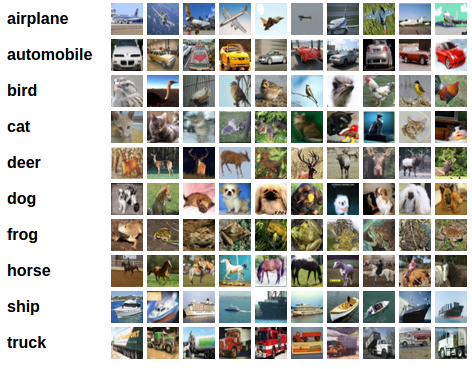
\includegraphics[width=\linewidth]{CIFAR.png}
\label{figure : CIFAR-10}
\end{figure}

\subsection{Gestione del Dataset}
Alla base della gestione dei \textit{Dataset} vi è la classe \textit{torch.utils.data.DataLoader}.
In Particolare tutti  sono sottoclassi di torch.utils.data.Dataset, ovvero hanno implementati i metodi \textit{getitem()} e \textit{len()}.
\newline
Per gestire il Dataset \textbf{CIFAR-10} ho istanziato nel mio progetto una classe \textit{Filtered\_dataset} che si occcupasse di questa mansione.
L'obbiettivo del mio elaborato era rappresentare il problema del \textbf{Continual Learning} e per fare ciò è necessario dividere il dataset utilizzato in \textit{Tasks}.
Ciò significa che a seconda del numero di \textit{Tasks} che io voglio utilizzare per simulare il \textbf{Continual Learning}
dovrò dividere il Dataset per \textit{Label}. Ad Esempio se io volessi utilizzare 5 \textit{Tasks}, per ognuno di essi avrei 2 \textit{Label}.\newline
La classe \textit{Filtered\_dataset} si occupa di creare un Subset con con il metodo della libreria di \textbf{PyTorch} \textit{torch.utils.data.Subset} che crea un subset del Dataset originario.\newline
Nel processo di suddivisione del Dataset è stato necessario \textit{mappare} le labels del dataset in modo tale da essere coerenti con l'output dell Rete. In particolare ciò è stato fatto tramite due attributi della classe \textit{Filtered\_dataset}:\textit{original2task} e \textit{task2original}. Questi due attributi consistono in due dizionari con chiave-valore le label e la rispettiva mappatura.
Ho reso inlotre possibile \textit{randomizzare} le label all'interno di ciascun task per poter fare ulteriori test con il metodo \textit{idx\_tasks}.
\newline
\section{Rete Neurale Convoluzionale}
La \textbf{Rete neurale Convoluzionale} (CNN o ConvNet) è una classe di \textit{Reti Neurali} profonde, molto spesso  applicata all'analisi ed al riconoscimento delle immagini.
La \textbf{Rete neurale Convoluzionale} che ho utilizzato in questo progetto è formata da sei \textit{Conv2D} layers separati da due \textit{MaxPool2D} ed infine da due \textit{Fully Connected Layer} sui cui ho applicato \textit{Dropout} per limitare l'\textit{Overfitting} durante il Training.
\newline
La particolarità di questa rete è che il layer dell'output è \textbf{\textit{Dinamico}}, cioè che cambia a seconda del numero di \textit{tasks} su cui si vuole lavorare e sulla tipologia di approccio scelto tra \textit{Task-Agnostic} e \textit{Task-Aware}.\newline
In Particolare è possibile aggiungere nuovi layer di output con il metodo\textit{add\_task} che richiama semplicemnte il metodo \textit{add\_module} della classe \textit{nn.Module}.
Un altro metodo importante della \textit{Rete Neurale} sarà  \textit{set\_tasks} che mi permette di settare il numero di tasks che voglio avere come output. I due attributi fondamentali della classe \textit{net} sono \textit{task\_fcs} e \textit{current\_tasks}, che sono sostanzialmente due Array contenenti gli indici dei \textit{tasks}. Il primo conterrà tutti i layer lineari per le varie  \textit{Classification Head}, mentre il secondo, seleziona quale(i) task(s) sono correntemente attivi.
Qui di seguito riporto la \textit{Rete Neurale} per un singolo task con tutte le classi corrispondente al \textit{Joint Training}:

\newline
Net(\\
  (conv1): Conv2d(3, 32, kernel_size=(3, 3), stride=(1, 1), padding=(1, 1))\\
  (conv2): Conv2d(32, 64, kernel_size=(3, 3), stride=(1, 1), padding=(1, 1))\\
  (conv3): Conv2d(64, 64, kernel_size=(3, 3), stride=(1, 1), padding=(1, 1))\\
  (pool): MaxPool2d(kernel_size=2, stride=2, padding=0, dilation=1, ceil_mode=False)\\
  (conv4): Conv2d(64, 128, kernel_size=(3, 3), stride=(1, 1), padding=(1, 1))\\
  (conv5): Conv2d(128, 128, kernel_size=(3, 3), stride=(1, 1), padding=(1, 1))\\
  (conv6): Conv2d(128, 256, kernel_size=(3, 3), stride=(1, 1), padding=(1, 1))\\
  (fc1): Linear(in_features=16384, out_features=120, bias=True)\\
  (fc2): Linear(in_features=120, out_features=84, bias=True)\\
  (dropout): Dropout(p=0.5, inplace=False)\\
  (task0\_fc): Linear(in_features=84, out_features=10, bias=True)\\
)
\newpage
Il layer \textit{Task0\_fc} è l'ultimo layer che è stato aggiunto con \textit{add\_task} e \textit{settato} con \textit{set\_task}.
Se l'esperimento fosse stato condotto su più \textit{Tasks} ci sarebbero stati altri layers oltre a \textit{Task0\_fc}. Nel caso in cui l'output voluto fosse stato su più tasks, nel metodo \textit{Forward} della rete tramite \textit{torch.cat}, sarebbero stati concatenati tra di loro i parametri corrispondenti selezionati da \textit{current\_tasks}.
\newline
La \textit{funzione di Attivazione} utilizzata nei layer \textit{Convoluzionali} è \textbf{ReLu}, come anticipato precedentemente.
La \textbf{rectified linear activation function} o \textbf{ReLU} in breve è una funzione lineare a tratti che darà  come output direttamente l'input se è positivo, altrimenti produrrà zero. L'utilizzo della \textbf{ReLu} consente di ottenere un \textit{Training} e una performance migliori.
\newline
Per quanto riguarda la funzione che si occupa del calcolo della \textit{Loss} ho optato per utilizzare la \textbf{CrossEntropyLoss}. Questa Funzione combina in una unica classe \textit{nn.LogSoftmax()} e \textit{ nn.NLLLoss()}.
Come anticipato nel paragrafo relativo a \textbf{PyTorch} ho utilizzato come \textit{optimizer} \textbf{SGD} con \textit{Learning Rate} pari a  \mathbf{0.001}.\newline
Infine, ho reputato necessario applicare \textbf{Dropout} ai due \textit{Fully Connected Layer} che precedono il layer di output dinamico. Durante il \textit{Training}, azzera in modo casuale alcuni degli elementi del tensore di input con probabilità p utilizzando campioni da una distribuzione di Bernoulli. In questo modo ho diminuito L'\textit{Overfitting}  riscontrato sulla \textit{Rete}.
\chapter{Conclusioni}\label{ch:conclusioni}
\ldots

\addcontentsline{toc}{chapter}{Bibliografia}
\bibliographystyle{plain}
\bibliography{files/biblio}
\bibliographystyle{unsrt}
%\bibliography{sp,xml}

\end{document} 